%-----------------------------------LICENSE------------------------------------%
%   This file is part of Mathematics-and-Physics.                              %
%                                                                              %
%   Mathematics-and-Physics is free software: you can redistribute it and/or   %
%   modify it under the terms of the GNU General Public License as             %
%   published by the Free Software Foundation, either version 3 of the         %
%   License, or (at your option) any later version.                            %
%                                                                              %
%   Mathematics-and-Physics is distributed in the hope that it will be useful, %
%   but WITHOUT ANY WARRANTY; without even the implied warranty of             %
%   MERCHANTABILITY or FITNESS FOR A PARTICULAR PURPOSE.  See the              %
%   GNU General Public License for more details.                               %
%                                                                              %
%   You should have received a copy of the GNU General Public License along    %
%   with Mathematics-and-Physics.  If not, see <https://www.gnu.org/licenses/>.%
%------------------------------------------------------------------------------%
%       Author: Ryan Maguire                                                   %
%       Date:   2021/11/16                                                     %
%------------------------------------------------------------------------------%
\documentclass{article}

% Needed for figures.
\usepackage{graphicx}

% Needed for mathbb font style.
\usepackage{amssymb}

% Tools for creating the theorem environment.
\usepackage{amsthm}

% The align environment is here.
\usepackage{amsmath}

% Library of colors, used here for displaying code.
\usepackage{xcolor}

% Used for displaying code in a LaTeX document.
\usepackage{listings}

% Used for correct hyperlinks with figures.
\usepackage[font={scriptsize}, hypcap=true, labelsep=colon]{caption}

% Hyperlinks for labels.
\usepackage{hyperref}

% Background color for code.
\definecolor{background}{rgb}{0.9, 0.9, 0.9}

% Display style used for the C programming language in this document.
\lstdefinestyle{CStyle}{
    backgroundcolor=\color{background},
    commentstyle=\color{gray},
    keywordstyle=\color{blue},
    numberstyle=\tiny\color{red},
    stringstyle=\color{orange},
    basicstyle=\footnotesize,
    breakatwhitespace=false,
    breaklines=true,
    captionpos=b,
    keepspaces=true,
    numbers=left,
    numbersep=5pt,
    showspaces=false,
    showstringspaces=false,
    showtabs=false,
    tabsize=2,
    language=C
}

% Display style for hyperlinks.
\hypersetup{
    colorlinks=true,
    linkcolor=blue
}

% Create a theorem environment, similar to most textbooks.
\theoremstyle{plain}
\newtheorem{theorem}{Theorem}

% No indent and no paragraph skip.
\setlength{\parindent}{0em}
\setlength{\parskip}{0em}

% Title page information.
\title{Conjectures on Legendrian and Transversally Simple Knots and Links and an
       Iterative Algorithm for the Jones' Polynomial}
\author{Vladimir Chernov\hspace{2em}Ryan Maguire}
\date{Fall 2021}

\begin{document}
    \maketitle
    \tableofcontents
    \begin{abstract}
        \noindent
        A theorem of Kronheimer and Mrowka states that Khovanov homology is
        able to detect the unknot \cite{kronheimermrowka2010}. That is, if a
        knot has the Khovanov homology of the unknot, then it is
        isomorphic to it. A similar result holds for Knot Floer
        homology. The unknot is the simplest of the torus knots, which is a
        class of knots known to be Legendrian simple. It is conjectured that
        Khovanov and Knot Floer homology are able to distinguish Legendrian
        and Transversally simple knot. An iterative algorithm for computing
        the Jones' polynomial of a knot is described and an analysis of the
        computational complexity is given. This algorithm is then used to
	efficiently compare the Khovanov homologies of all knots of up to 13
	crossings with all torus knots of up to 50 crossings, providing
	numerical evidence for this conjecture on the first $\approx12,000$
	knots.
    \end{abstract}
    \section{Extended Gauss Code}
        Given a knot diagram, it is reasonable for a mathematician to wish to
        describe the figure with finite data in such a way that a computer can
        understand and perform computations. This is achieved via Gauss code.
        Orient the knot, label the crossings, and choose a starting point.
        Walk along the diagram, following the orientation, and record the
        crossings. That is, write down the crossing number, and whether the
        the path goes under or over the crossing with a $U$ or $O$,
        respectively. This is illustrated via example for the right-handed
        trefoil knot in Fig.~\ref{fig:right_handed_trefoil_gauss_code}.
        \begin{figure}
            \centering
            \includegraphics{%
                ../images/trefoil_knot_oriented_with_gauss_code.pdf%
            }
            \caption{Gauss Code for the Right-Handed Trefoil}
            \label{fig:right_handed_trefoil_gauss_code}
        \end{figure}
        Gauss code is not unique to a knot diagram since the code is dependent
        on the choice of starting point. This causes two different issues.
        First, when trying to determine if two knots are the same, we must
        check if one Gauss code is a cyclic permutation of another. Secondly,
        and more importantly, this version of Gauss code cannot distinguish
        between a knot and its mirror. If we take the left-handed trefoil,
        give it a similar orientation as before, but choose a different
        starting point, we end up with
        Fig.~\ref{fig:left_handed_trefoil_gauss_code}. The resulting Gauss code
        is the same as the Gauss code we get for the right-handed trefoil.
        These are different knots since they have different Jones' polynomials,
        meaning Gauss code cannot distinguish mirrors.
        \begin{figure}
            \centering
            \includegraphics{%
                ../images/trefoil_knot_mirror_oriented_with_gauss_code.pdf%
            }
            \caption{Gauss Code for the Left-Handed Trefoil}
            \label{fig:left_handed_trefoil_gauss_code}
        \end{figure}
        The solution is to \textit{sign} the crossings. Given an oriented knot,
        we label a crossing positive or negative depending on which strand is
        over and which is under. This is shown in Fig.~\ref{fig:crossing_signs}.
        \begin{figure}
            \centering
            \includegraphics{../images/crossing_signs.pdf}
            \caption{Crossing Signs}
            \label{fig:crossing_signs}
        \end{figure}
        By keeping track of the sign we get extended Gauss code
        (also called signed Gauss code).
        \begin{figure}
            \centering
            \includegraphics{%
                ../images/trefoil_knot_oriented_with_extended_gauss_code.pdf%
            }
            \caption{Extended Gauss Code for the Right-Handed Trefoil}
            \label{fig:right_hand_trefoil_extended_gauss}
        \end{figure}
        Note the orientation does not matter. If we reverse the orientation,
        the signs are still preserved. Examine Fig.~\ref{fig:crossing_signs} to
        convince yourself of this.
        \par\hfill\par
        Computationally, Extended Gauss code is a finite sequence of ordered
        triples. The length of the sequence is $2N$ where $N$ is the number of
        crossings in the diagram, and the ordered triples are of the form
        $(t,n,s)$ where $t\in\{O,U\}$, $s\in\{+1,-1\}$, and
        $0\leq{n}\leq{N-1}$ ($t$ for \textit{type}, $s$ for \textit{sign}, and
        $n$ for indexing). One could represent this in the C programming
        language as follows.
        \begin{lstlisting}[style=CStyle, gobble=12]
            enum crossing_sign {negative_crossing, positive_crossing};
            enum crossing_type {under_crossing, over_crossing};

            struct knot {
                unsigned int number_of_crossings;
                enum crossing_sign *sign;
                enum crossing_type *type;
                unsigned int *crossing_number;
            };
        \end{lstlisting}
        The pointers to the arrays \texttt{sign}, \texttt{type}, and
        \texttt{crossing\_number} each having 2 times
        \texttt{number\_of\_crossings} many elements.
        Similar definitions could easily be given with classes using the
        Python programming language. Regardless of preference, we now have a
        means of representing a knot in a computer.
    \section{Virtual Knots}
        Not all finite sequences of length $2N$ will be valid Gauss code. For
        the code to be valid every integer $0\leq{n}\leq{N-1}$ must occur
        exactly twice, once with $t=O$ and once with $t=U$, and the sign
        $s$ must be the same for both crossings. Consider the following Gauss
        code:
        \begin{equation}
            O0+O1+U0+U1+
        \end{equation}
        It satisfies the above criterion.
        The code tells us we have a two crossing knot. A quick look through any
        table of knots tells us the smallest number of crossings a non-trivial
        knot can have is 3 (the left and right trefoils). The
        Reidemeister moves can translate to operations on extended Gauss code,
        but you'll find they're of no help here. Let's try to draw it
        (Fig.~\ref{fig:chain_link_fence_knot}).
        \begin{figure}
            \centering
            \includegraphics{../images/chain_link_fence_knot_virtual.pdf}
            \caption{The Chain Link Fence Knot}
            \label{fig:chain_link_fence_knot}
        \end{figure}
        To do this on a piece of paper requires us to pretend one crossing is
        fake, or \textit{virtual}. Graph theory tells us we really want to draw
        this on a higher genus surface. Using the torus $\mathbb{T}^{2}$ we can
        draw this knot without virtual crossings
        (Fig.~\ref{fig:chain_link_fence_knot_on_torus}). This will be called
        the \textit{chain-link-fence} knot. The name makes sense if we draw it
        on the flat torus (Fig.~\ref{fig:chain_link_fence_knot_on_flat_torus}).
        \begin{figure}
            \centering
            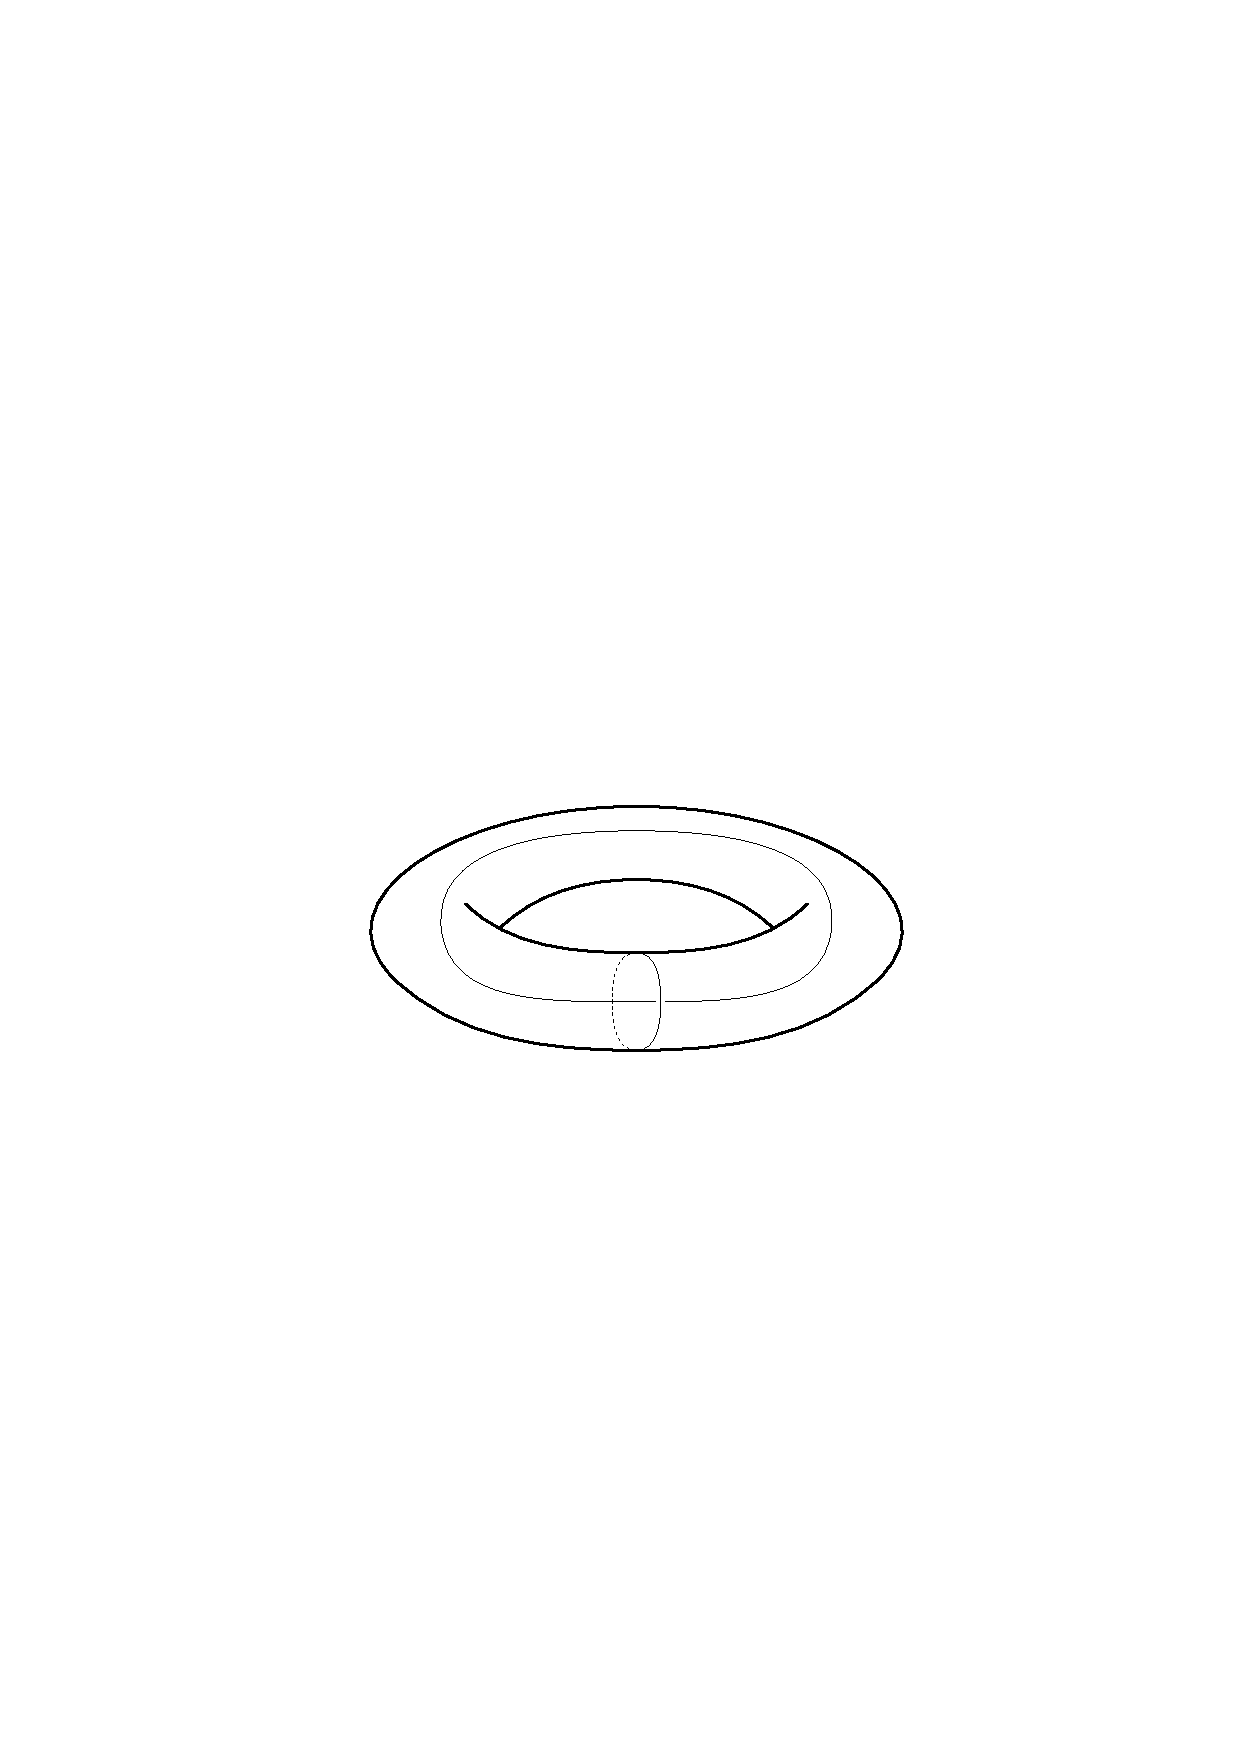
\includegraphics{../images/chain_link_fence_knot_on_torus.pdf}
            \caption{The Chain Link Fence Knot on a Torus}
            \label{fig:chain_link_fence_knot_on_torus}
        \end{figure}
        \begin{figure}
            \centering
            \includegraphics{../images/chain_link_fence_knot_on_flat_torus.pdf}
            \caption{The Chain Link Fence Knot on a Flat Torus}
            \label{fig:chain_link_fence_knot_on_flat_torus}
        \end{figure}
        Lifting this drawing to the universal cover, we see a chain-link fence
        (Fig.~\ref{fig:chain_link_fence_knot_on_flat_torus_universal_cover}).
        Such objects are called \textit{virtual knots}, knots that can be
        embedded into some 3-manifold of the form $M\times\mathbb{R}$ where
        $M$ is a smooth surface. Given the Gauss code of a virtual knot, if your
        drawing requires you to have $m$ virtual crossings, you could embed the
        knot diagram into the compact surface $M$ of genus $m$. At every virtual
        crossing you add a handle, removing the crossing. The result is an
        embedding of the diagram onto $M$, meaning the virtual knot could be
        embedded into $M\times\mathbb{R}$. This idea is a
        mimicry of the proof that every graph can be embedded onto some surface.
        A classical knot is a virtual knot that can be embedded into
        $\mathbb{S}^{2}\times\mathbb{R}$. The chain-link-fence knot is the
        simplest non-trivial virtual knot. There are no virtual knots with one
        crossing (but there are virtual \textit{links} with one crossing). This
        is useful for test computations.
        \begin{figure}
            \centering
            \resizebox{\textwidth}{!}{%
                \includegraphics{%
                    ../images/chain_link_fence_knot_on_flat_torus_universal_cover.pdf%
                }%
            }
            \caption{Lift of the Chain Link Fence Knot to $\mathbb{R}^{2}$}
            \label{fig:chain_link_fence_knot_on_flat_torus_universal_cover}
        \end{figure}
    \section{Resolving a Crossing}
        The Kauffman bracket polynomial is an invariant for
        \textit{framed links}. It is not a link invariant since the polynomial
        is not preserved by Reidemeister I moves (though this can be salvaged
        by a proper normalization, resulting in the Jones' polynomial). The
        definition we'll give in the next section is similar to the
        description provided in \cite{barnatan2002khovanov}. It is recursive
        and requires us to \textit{resolve crossings}. Resolving a crossing
        equates to removing it. There are two ways to do this.
        Given an unoriented knot diagram, we rotate our heads until
        the over crossing travels from the top left to the bottom right. The
        0 and 1 resolution of the crossing are given in
        Fig.~\ref{fig:resolving_crossing}.
        \begin{figure}
            \centering
            \includegraphics{../images/resolving_crossings.pdf}
            \caption{Resolving a Crossing}
            \label{fig:resolving_crossing}
        \end{figure}
        Given the Gauss code of a knot diagram with $N$ crossings, and a number
        $0\leq{n}\leq{2}^{N}-1$, there is a unique resolution of all of the
        crossings corresponding to $n$. Write $n$ in binary. The value of the
        $k^{th}$ bit in the binary representation of $n$ corresponds to how the
        $k^{th}$ crossing is smoothed. Examine the right-handed trefoil with its
        standard knot diagram (Fig.~\ref{fig:right_handed_trefoil_gauss_code}).
        There are 3 crossings, so $2^{3}=8$ possible resolutions. The diagram
        in Fig.~\ref{fig:trefoil_knot_cube_of_resolutions} is called the
        \textit{cube of resolutions} for the right-handed
        trefoil. This language is slightly misleading since the cube of
        resolutions is dependent on the knot diagram, so it is better to say
        this is the cube of resolutions for the \textit{standard} diagram of
        the right-handed trefoil. The image gets complicated quickly since the
        size of the cube is exponential in the number of crossings. The cube of
        resolutions for the figure-eight knot is shown in
        Fig.~\ref{fig:figure_eight_knot_cube_of_resolutions}.
        \begin{figure}
            \centering
            \includegraphics{../images/trefoil_knot_cube_of_resolutions.pdf}
            \caption{Cube of Resolutions for the Left-Handed Trefoil}
            \label{fig:trefoil_knot_cube_of_resolutions}
        \end{figure}
        \begin{figure}
            \centering
            \resizebox{\textwidth}{!}{%
                \includegraphics{%
                    ../images/figure_eight_knot_cube_of_resolutions.pdf%
                }%
            }
            \caption{Cube of Resolutions for the Figure-Eight}
            \label{fig:figure_eight_knot_cube_of_resolutions}
        \end{figure}
        Connecting the appropriate images with arrows results in a tesseract.
        For neatness, this has been omitted.
    \section{The Kauffman Bracket}
        The Kauffman bracket polynomial of a link $L$ is defined recursively
        in terms of smoothings of a link diagram. The definition is:
        \begin{align}
            \langle\emptyset\rangle&=1\\
            \langle{L\sqcup\mathbb{S}^{1}}\rangle&=(q+q^{-1})\langle{L}\rangle\\
            \langle{L}\rangle&=
                \langle{L_{n,0}}\rangle-q\langle{L_{n,1}}\rangle
        \end{align}
        where $L_{n,0}$ and $L_{n,1}$ are the links obtained from the
        0 and 1 smoothings of $L$ at the $n^{th}$ crossing, respectively. The
        notation $L\sqcup\mathbb{S}^{1}$ means the disjoint union of
        $L$ with an unknot. Hence the Kaufmann bracket of the
        unknot is $q+q^{-1}$.
        \par\hfill\par
        The third equation reduces an $N$ crossing link to two $N-1$ crossing
        links. If we continue this recursive step we'll end up with
        $2^{N}$ completely resolved links, each being the disjoint union of
        circles. Applying the first and second equations, we can inductively
        prove the following formula for the Kauffman bracket:
        \begin{equation}
            \label{eqn:kauffman_bracket}%
            \langle{L}\rangle=\sum_{n=0}^{2^{N}-1}
                (-q)^{w(n)}(q+q^{-1})^{c(n)}
        \end{equation}
        Here, $w(n)$ is the Hamming weight of $n$, the number of 1's
        that occur in the binary expansion of $n$. Recalling that an integer
        $0\leq{n}\leq{2}^{N}-1$ represents a complete smoothing of a knot,
        $c(n)$ is the number of circles that result from the $n$ smoothing.
        The Hamming weight is a well studied function and efficient methods of
        computing it are known, including constant-time algorithms if one
        restricts their attention to fixed-width integers
        (usually 32 or 64 bit). A general and portable algorithm can be done in
        $\log(n)$ time as follows.
        \begin{lstlisting}[style=CStyle, gobble=12]
            static unsigned int hamming_weight(unsigned int val)
            {
                unsigned int result = 0U;

                while(val != 0U)
                {
                    result += val & 1U;
                    val = val >> 1U;
                }

                return result;
            }
        \end{lstlisting}
        The code \texttt{result += val \& 1U} may need explanation.
        \texttt{val \& 1U} performs a bitwise \texttt{AND} with \texttt{val} and
        1. Since the binary representation of 1 is zero in all slots except the
        zeroth bit, \texttt{val \& 1U} is simply checking the zeroth bit of
        \texttt{val}. We add this value to \texttt{result}, ultimately giving
        us the Hamming weight. The code \texttt{val = val >> 1U} takes val and
        shifts it 1 bit to the right. So, if we had $111_{2}$ and shift it to
        the right, we'd end up with $011_{2}$. Because of this, after
        \texttt{log(val)} steps \texttt{val} would be zero, exiting the
        while-loop.
        \par\hfill\par
        For the Kauffman bracket this function is used with inputs of size
        $2^{N}-1$, where $N$ is the number of crossings, so the worst-case
        time complexity at this step is $O(N)$. For example, considering the
        resolution of the right-handed trefoil
        in Fig.~\ref{fig:right_hand_trefoil_extended_gauss} corresponding to
        $7=111_{2}$, the loop will end after 3 steps, one step for each
        crossing. The $000_{2}$ resolution exits immediately.
        \par\hfill\par
        With the Hamming weight settled, the remaining information needed to
        compute the Kauffman bracket is the number of circles that result from
        the $n^{th}$ smoothing ($0\leq{n}\leq{2}^{N}-1$). This paper gives a
        simple algorithm using extended Gauss code. The code outlined works for
        knots, but simple extensions could be made for links. In particular, the
        algorithm works for \textit{virtual knots} and there is no restriction
        to the classical setting.
    \section{The Circle Counting Algorithm}
        The visual for the algorithm goes as follows. Given a knot, we thicken
        it into a framed knot (Fig.~\ref{fig:trefoil_knot_framed_001}). Every
        crossing becomes a four-way intersection
        (Fig.~\ref{fig:thickened_crossings}), and the idea is to loop
        over then $4N$ roads in this thickened knot, $N$ being the number of
        crossings. We first examine the negative crossing. The 0 and 1
        smoothings are shown in
        Fig.~\ref{fig:thickened_negative_crossing_smoothings}. Suppose we start
        on the bottom-left road of the 0-smoothing and walk towards the
        crossing. The smoothing in the visual equates to a road block, the thick
        black line we are unable to pass through. We are thus forced to go down
        the bottom-right road. The arrow for this road is going the wrong way,
        pointing towards the crossing and we are moving away from it.
        To preserve orientation we must walk backwards. This
        translates as follows for extended Gauss code. Approaching a negative
        crossing from the bottom left road means we have approached $Un-$ in
        the code reading left-to-right, $n$ being the crossing number. The
        road block tells us to go down the bottom right road, but in reverse.
        That is, look for $On-$ in the code and then go
        to the \textit{previous} entry in the code.
        This is equivalent to walking backwards. We end up at a new crossing.
        We now know the rule for approaching a crossing from the bottom left
        road for a negative crossing given the 0-smoothing. In total there are
        16 possible cases: Is the sign $+1$ or $-1$, is the type $U$ or $O$, is
        the smoothing $0$ or $1$, is the direction forwards or backwards. The
        visuals for these 16 combinations are shown in
        Fig.~\ref{fig:thickened_negative_crossing_smoothings} and
        Fig.~\ref{fig:thickened_positive_crossing_smoothings}.
        \par\hfill\par
        \begin{figure}
            \centering
            \includegraphics{../images/trefoil_knot_framed_001.pdf}
            \caption{Framed Left-Handed Trefoil}
            \label{fig:trefoil_knot_framed_001}
        \end{figure}
        \begin{figure}
            \centering
            \includegraphics{../images/thickened_crossings.pdf}
            \caption{Signed Crossings in a Framed Knot}
            \label{fig:thickened_crossings}
        \end{figure}
        \begin{figure}
            \centering
            \includegraphics{../images/thickened_negative_crossing_smoothings.pdf}
            \caption{Smoothing a Negative Crossing in a Framed Knot}
            \label{fig:thickened_negative_crossing_smoothings}
        \end{figure}
        \begin{figure}
            \centering
            \includegraphics{../images/thickened_positive_crossing_smoothings.pdf}
            \caption{Smoothing a Positive Crossing in a Framed Knot}
            \label{fig:thickened_positive_crossing_smoothings}
        \end{figure}
        Jumping from the over-crossing to the under-crossing, and vice-verse,
        as is needed in the algorithm is made easier if we have an array
        \texttt{ind} such that \texttt{ind[n]} is an ordered pair whose
        zeroth entry is the index of the under-crossing for the $n^{th}$
        crossing, and first entry is the index of the over-crossing. It is then
        useful to describe a \texttt{struct} for this ordered pair, and an
        algorithm to obtain this array.
        \begin{lstlisting}[style=CStyle, gobble=12]
            struct CrossingIndices {
                unsigned int under;
                unsigned int over;
            };

            static struct CrossingIndices *get_indices(struct knot *K)
            {
                unsigned int n;
                struct CrossingIndices *ind;

                if (!K)
                    return NULL;

                if (K->number_of_crossings == 0U)
                    return NULL;

                ind = malloc(sizeof(*ind)*K->number_of_crossings);

                if (!ind)
                    return NULL;

                for (n = 0U; n < 2U * K->number_of_crossings; ++n)
                {
                    if (K->type[n] == over_crossing)
                        ind[K->crossing_number[n]].over = n;
                    else
                         ind[K->crossing_number[n]].under = n;
                }

                return ind;
            }
        \end{lstlisting}
        The error checks are for good programming practice: Check if your
        input pointer is \texttt{NULL}, don't assume \texttt{malloc} was
        successful, and don't pass zero to \texttt{malloc}. The actual algorithm
        is contained in the for loop. We loop over the Gauss code, ask which
        crossing number we have, and then add this index to our array. The
        loop requires $2N$ steps, $N$ being the number of crossings, so this
        step is $O(N)$. Unlike the Hamming weight and the number of circles
        from a resolution, this index-finding algorithm is only needed once. We
        execute the algorithm at the start and then store the result in
        memory.
        \par\hfill\par
        Because of the 16 possibilities, the full algorithm is lengthy. To make
        this easier we label the roads so that we can make a table. This is
        done in Fig.~\ref{fig:thickened_crossings_labeled}. By examining
        Fig.~\ref{fig:thickened_crossings_resolved_labeled} we can tell where
        we need to go as we walk along the knot. This is done explicitly in
        Tab.~\ref{tab:circle_counting_algorithm_where_go}. The table reads as follows.
        The left \textit{In} column tells you which road you are approaching the
        crossing from. Note if you are approaching from roads 0 or 1, you are
        walking forward, and if you are approaching from roads 2 or 3, you are
        walking backwards. Using the information about the sign and resolution
        of the crossing, you know which road to leave from. In the Gauss code,
        if you approach an under crossing, find the corresponding over crossing
        in the code (and vice-versa). Then go to the previous entry if you are
        leaving from roads 0 and 1, and the next entry if leaving from roads
        2 or 3. Eventually you will return to an entry in
        the Gauss code you have already been to. This amounts to 1 circle from
        the resolution. Move on to the next element of the Gauss code you have
        yet to encounter and repeat. Tab.~\ref{tab:circle_counting_algorithm_where_start}
        then tells which road number you are entering based on the sign and type
        of the crossing, and the direction you are walking. Eventually the code
        will be exhausted, and the resulting tally is the number of
        circles from this resolution.
        \begin{figure}
            \centering
            \includegraphics{../images/thickened_crossing_labeled.pdf}
            \caption{Thickened Crossings with Labels}
            \label{fig:thickened_crossings_labeled}
        \end{figure}
        \begin{figure}
            \centering
            \includegraphics{../images/thickened_crossings_resolved_labeled.pdf}
            \caption{Thickened Resolved Crossings with Labels}
            \label{fig:thickened_crossings_resolved_labeled}
        \end{figure}
        \begin{table}
            \centering
            \begin{tabular}{c c c c}
                Type&Sign&Direction&In\\
                \hline
                $O$&-&Forward&1\\
                $O$&-&Backward&3\\
                $O$&+&Forward&0\\
                $O$&+&Backward&2\\
                \hline
                $U$&-&Forward&0\\
                $U$&-&Backward&2\\
                $U$&+&Forward&1\\
                $U$&+&Backward&3
            \end{tabular}
            \caption{The Circle Counting Algorithm - Where to Start}
            \label{tab:circle_counting_algorithm_where_start}
        \end{table}
        \begin{table}
            \centering
            \begin{tabular}{c c c c}
                In&Sign&Resolution&Out\\
                \hline
                0&-&0&1\\
                0&-&1&3\\
                0&+&0&3\\
                0&+&1&1\\
                \hline
                1&-&0&0\\
                1&-&1&2\\
                1&+&0&2\\
                1&+&1&0\\
                \hline
                2&-&0&3\\
                2&-&1&1\\
                2&+&0&1\\
                2&+&1&3\\
                \hline
                3&-&0&2\\
                3&-&1&0\\
                3&+&0&0\\
                3&+&1&2
            \end{tabular}
            \caption{The Circle Counting Algorithm - Where to Go}
            \label{tab:circle_counting_algorithm_where_go}
        \end{table}
        \par\hfill\par
        Let's use the trefoil as an example. The $000_{2}$ resolution results
        in 2 circles (Fig.~\ref{fig:trefoil_knot_cube_of_resolutions}). Let's
        check that the algorithm detects this. The Gauss code is
        $O0+U1+O2+U0+O1+U2+$. We start by entering the zeroth crossing
        (road 0). It is an over crossing, so we look ahead in the code and
        find the corresponding under crossing. It is a positive crossing with
        the zero resolution, so Tab.~\ref{tab:circle_counting_algorithm_where_go} tells
        us to leave through road 3. We mark road 0 and road 3 of the zeroth
        crossing as travelled and proceed. Leaving through road 3 means we
        travel forward. Hence we wind up at $O1+$ in the code and we are
        walking forwards. Over-crossing, positive sign, walking forwards means
        we are entering the crossing from road 0
        (Tab.~\ref{tab:circle_counting_algorithm_where_start}). We will again
        leave through road 3 and enter the $O2+$ crossing walking forwards.
        We again enter road 0 and leave through road 3 and wind up at
        $O0+$ walking forward, completing our first cycle. The next untouched
        road is road 1 for the zeroth crossing. This corresponding to $U0+$
        walking forwards. Tab.~\ref{tab:circle_counting_algorithm_where_go}
        tells us to leave through road 2. We end up at $U1+$ at road 1. Again
        we leave through road 2 and end up at $U2+$ road 1. We leave through
        road 3 entering $U0+$, completing our cycle. All of the roads have been
        marked, and we have 2 circles total, in agreement with
        Fig.~\ref{fig:trefoil_knot_cube_of_resolutions}.
        \par\hfill\par
        To compute the Kauffman bracket, we loop over all integers
        $0\leq{n}\leq{2}^{N}-1$, $N$ being the number of crossings, compute the
        number of circles corresponding to the $n$ resolution using this
        algorithm, and perform the sum in Eqn.~\ref{eqn:kauffman_bracket}. The
        circle counting algorithm requires $4N$ steps since we loop over the
        $4N$ roads, and the Hamming weight has worst-case complexity $O(N)$,
        meaning each stage is $O(4N)+O(N)=O(N)$ in time complexity. There are
        $2^{N}$ total steps, so $O(N2^{N})$ is the total complexity of the
        computation. The computation of the array of indices at the beginning
        is $O(N)$, but as mentioned is only required once and is not part of
        the inner for-loop. The result for the entire algorithm is
        $O(N+N2^{N})=O(N2^{N})$. This is the same complexity as most useable
        algorithms. There are known algorithms in time $O(2^{C\sqrt{n}})$ for a
        constant $C$, but the constant is large enough that the algorithm is
        not feasible for most knots.
        \par\hfill\par
        To obtain the unnormalized Jones' polynomial we simply need to shift
        the degree of the resulting Kauffman bracket polynomial. This is
        defined by:
        \begin{equation}
            \tilde{J}(L)=(-1)^{N_{-}}q^{N_{-}-2N_{+}}\langle{L}\rangle
        \end{equation}
        Where $N_{-}$ is the number of negative crossings and $N_{+}$ is the
        number of positive crossings. We represent Laurent polynomials by the
        following struct:
        \begin{lstlisting}[style=CStyle, gobble=12]
            struct laurent_polynomial {
                signed int lowest_degree;
                signed int highest_degree;
                signed int *coeffs;
            };
        \end{lstlisting}
        The $q^{N_{-}-2N_{+}}$ term thus takes $O(1)$ in time, we simply
        add $N_{-}-2N_{+}$ to \texttt{highest\_degree} and
        \texttt{lowest\_degree}. This step does not impact the computation time
        in any significant way.
        \par\hfill\par
        The main benefit is that the algorithm is \textit{iterative} instead of
        recursive. The complexity is bad enough that the recursive
        algorithms may result in stack overflows. Such is the case with some of
        the Python packages that exist to compute the Jones' polynomial. The
        computation of the Jones' polynomial of a 30 crossing knot results in
        runtime errors do to too many recursions. With infinite memory, 30
        crossing knots could have their Jones' polynomials computed na\"{i}vely
        in about a day or so if one wishes to wait that long. The benefit of
        this iterative method is that it requires only $O(N)$ space,
        not $O(2^{N})$, so infinite memory isn't needed. One could hit
        \textit{go} and wait a day and then have the Jones' polynomial of their
        knot.
    \section{Results}
        A theorem of Mrowka and Kronheimer states that the Khovanov homology
        detects the unknot. That is, if a given knot has the same Khovanov
        homology as the unknot, then that knot \textit{is} the unknot.
        The unnormalized Jones' polynomial is the graded Euler characteristic of
        Khovanov homology, so it has been conjectured that the Jones's
        polynomial also detects the unknot. This is currently unknown. The
        algorithm described here has been used, in combination with the
        Python packages \texttt{snappy} and \texttt{regina}, to look for
        numerical evidence of stronger conjectures. The unknot is the simplest
        of the torus knots, so a natural generalization is
        \textit{does the Jones' polynomial distinguish torus knots}? That is,
        if a knot has the same Jones' polynomial as a torus knot, is that knot
        a torus knot itself? The answer is no via counterexample. Just in the
        Rolfsen table, the $10_{132}$ knot matches in $T(2,5)$ torus knot.
        Beyond the Rolfsen table, the 12 crossing knot K12n749 has the same Jones'
        polynomial as the the torus knot $T(2,7)$. In both instances the
        Khovanov homologies were different, leading to the following conjecture:
        \textit{Does Khovanov homology distinguish torus knots?} This is a
        natural generalization of Kronheimer and Mrowka's theorem, and there is
        supporting evidence amongst the first 2,977 knots (all knots of less
        than or equal to 12 crossings).
        The unknot is also the simplest of the twist knots. A modification of
        the Jones' polynomial conjecture for the unknot is whether the Jones'
        polynomial distinguishes twist knots. This is also false, but the first
        counterexamples don't occur until 11 crossings. These knots are
        described in Tab.~\ref{tab:counterexamples_twist_knot_conjecture}. Since
        a twist knot can be described by a single integer (the number of twists)
        the integers in the right column of this table show which twist knot
        matched a given knot in the HT non-alternating table. Two 12 crossing
        knots were also found, the knot K12a803 matches the $m_{10}$ twist knot,
        and the knot K12n475 matches $m_{3}$. The Khovanov homologies were
        computer for the knots in the HT non-alternating table and were found
        to be different than the twist knots, leading to another generalized
        conjecture: \textit{Does Khovanov homology distinguish twist knots}?
        \begin{table}
            \centering
            \begin{tabular}{c | c}
                HT Table&Twist Knot\\
                \hline
                K11n13&$m_{7}$\\
                K11n19&$m_{2}$\\
                K11n57&$m_{3}$\\
                K11n70&$m_{6}$\\
                K11n88&$m_{5}$
            \end{tabular}
            \caption{Counterexamples to Twist-Knot Conjecture}
            \label{tab:counterexamples_twist_knot_conjecture}
        \end{table}
    \newpage
    \bibliographystyle{plain}
    \bibliography{../biblio.bib}
    \newpage
    The source code used to generate this document is free software and released
    under version 3 of the GNU General Public License.
\end{document}

